\chapter{Novel Datasets for Transfer Learning}

\begin{remark}{Outline}

This chapter ...

\vspace{5mm}
\textit{This chapter is based on the publication \citet{sabatelli2021advances}.}
\label{ch:minerva_paper}


\end{remark}


\section{Challenges of Modern Computer Vision}
\label{sec:cv_challenges}


\subsection{Photo-realism}
\subsection{Data Scarcity}
\subsection{Irrelevant Training Categories}
\subsection{Model Robustness}



\section{The MINERVA Dataset}
\label{sec:minerva_dataset}

\subsection{Music Iconography}
\subsection{Data Collection}
\subsection{Annotation Process}
\subsection{Versions and Splits}

\begin{tabular}{l|rr|rr|rr} \hline
	$\mathcal{T}_T$ &  \multicolumn{2}{c}{training-set} & \multicolumn{2}{|c|}{validation-set} & \multicolumn{2}{c}{testing-set}\\
& $N_t$ & $I_t$ & $N_t$ & $I_t$ & $N_t$ & $I_t$ \\\hline \hline
\texttt{Minerva-0} & 1857 & 4243 & 1137 & 2288 & 1182 & 2102 \\
\texttt{Minerva-5} & 952 & 1589 & 540 & 852 & 721 & 1173\\
\texttt{Minerva-10} & 1227 & 2147  & 680 & 1127 & 897 & 1506 \\
\hline

\end{tabular}


\begin{figure}[htb!]
	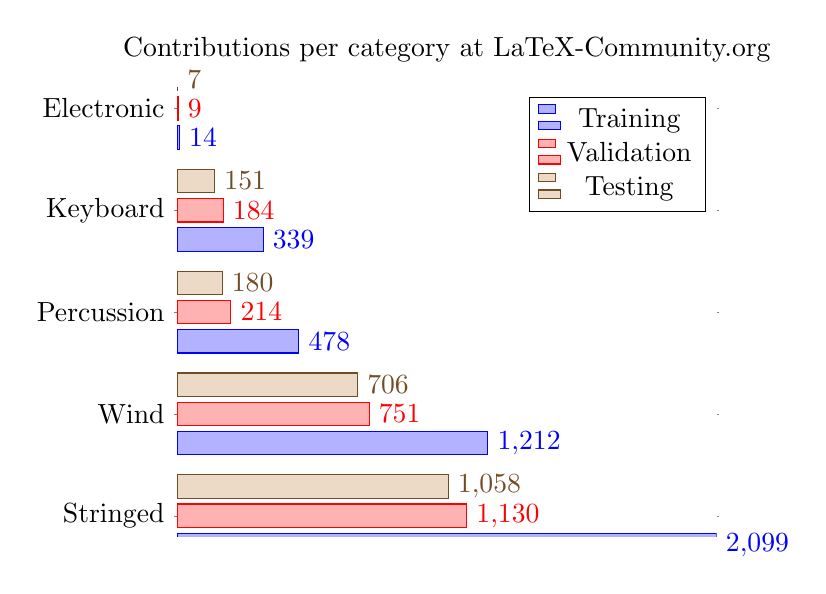
\begin{tikzpicture}
  \begin{axis}[title  = Contributions per category
                          at LaTeX-Community.org,
    xbar,
    bar width=.3cm,
    y axis line style = { opacity = 0 },
    axis x line       = none,
    tickwidth         = 1pt,
    enlarge y limits  = 0.05,
    enlarge x limits  = 0.001,
    symbolic y coords = {Stringed, Wind, Percussion,Keyboard, Electronic},
    nodes near coords,
  ]
\addplot coordinates {(2099,Stringed) (1212,Wind) (478,Percussion) (339,Keyboard) (14,Electronic)};
\addplot coordinates {(1130,Stringed) (751,Wind) (214,Percussion) (184,Keyboard) (9,Electronic)};
\addplot coordinates {(1058,Stringed) (706,Wind) (180,Percussion) (151,Keyboard) (7,Electronic)};
\legend{Training,Validation,Testing}

\end{axis}
\end{tikzpicture}

\iffalse
\end{axis}
\end{tikzpicture}
\fi

	\caption{}
	\label{fig:hypernym_distribution}
\end{figure}



\section{Benchmarking}
\label{sec:benchmarking}

\subsection{Classification}
\subsection{Object Detection}


\section{Results}
\label{sec:results}

\subsection{Quantitative Analysis}
\paragraph{Classification}
\paragraph{Object Detection}

\subsection{Qualitative Analysis}
\paragraph{True vs False Positives}
\paragraph{Saliency Maps}


\section{Discussion and Critical Analysis}
\label{sec:discussion}


\section{Future Work: towards more benchmarks}
\label{sec:future_work}
